\documentclass[11pt,a4paper]{article}

\usepackage[margin=2.4cm]{geometry}
\usepackage{amsmath,amssymb}
\usepackage{siunitx}
\usepackage{booktabs}
\usepackage{graphicx}
\usepackage{array}
\usepackage{caption}
\usepackage[table]{xcolor}
\usepackage{enumitem}
\usepackage[hidelinks]{hyperref}
\usepackage{fancyhdr}

\definecolor{ink}{HTML}{14202B}
\definecolor{accent}{HTML}{1D4ED8}
\definecolor{heat}{HTML}{EA580C}
\definecolor{rulegrey}{HTML}{C7D0D8}

\captionsetup{font=small,labelfont=bf,labelsep=period}
\setlength{\parskip}{0.5em}
\setlength{\parindent}{0pt}
\renewcommand{\arraystretch}{1.25}

\pagestyle{fancy}
\fancyhf{}
\lhead{\small\color{ink}ThermoTwin: Fired-Heater Digital Twin}
\rhead{\small\color{ink}Technical reference}
\cfoot{\small\thepage}
\renewcommand{\headrulewidth}{0.4pt}

\begin{document}

%============================ TITLE ============================
\begin{titlepage}
\vspace*{2cm}
{\color{accent}\rule{\textwidth}{2pt}}\\[0.4cm]
{\Huge\bfseries\color{ink} ThermoTwin}\\[0.3cm]
{\LARGE\color{ink} A First-Principles Digital Twin for Refinery Fired Heaters}\\[0.5cm]
{\large\color{ink} Governing equations, data generation, surrogate model and optimizer}\\[0.3cm]
{\color{heat}\rule{\textwidth}{2pt}}\\[0.9cm]

{\large\bfseries\color{ink} Abhishek Chankapure \quad\textbullet\quad Saurabh Ramteke \quad\textbullet\quad Vaibhav Patil}\\[0.2cm]
{\color{ink} trio team, IIT Madras (Chemical Engineering and Machine Learning)}\\[1.1cm]

{\large This document states every equation used in the project, the assumptions
behind them, and how the pieces fit together, so that a new reader can follow the
work from the combustion chemistry to the final fuel and carbon savings.}\\[1.5cm]

\begin{tabular}{@{}ll@{}}
\textbf{Project} & Physics + machine-learning twin for fired-heater optimization\\
\textbf{Team} & trio: Abhishek Chankapure, Saurabh Ramteke, Vaibhav Patil\\
\textbf{Source specification} & \texttt{HEATER KPIs.xlsx} (roadmap, compositions, KPI formulas)\\
\textbf{Code} & \texttt{C:\textbackslash trio\textbackslash heater\_sim}\\
\textbf{Status} & Prototype validated on first-principles simulation\\
\end{tabular}

\vfill
{\small All quantities use SI units unless stated. Heating values are lower
heating values at \SI{25}{\celsius} unless marked HHV.}
\end{titlepage}

\tableofcontents
\newpage

%============================ 1. OVERVIEW ============================
\section{What this project does}

A fired heater burns fuel gas to raise the temperature of a process stream. It is
the largest single fuel user and carbon source on a refinery unit. The heater
runs with extra combustion air as a safety margin against incomplete burning, and
that extra air carries heat up the stack, which wastes fuel. The safe optimum
moves with fuel composition, throughput, fouling and weather, so a static setting
is never optimal for long.

ThermoTwin is a digital twin of the heater. It has three layers:

\begin{enumerate}[leftmargin=1.4em]
  \item A \textbf{first-principles model} that closes the combustion and energy
        balance from physics alone. It needs no plant history, so it is useful on
        the first day of a deployment (Sections \ref{sec:fuel}--\ref{sec:kpi}).
  \item A \textbf{data generator} that drives the model through a realistic
        operating history with drift and labelled faults, producing a dataset
        that stands in for a plant historian at the ideation stage
        (Section \ref{sec:data}).
  \item A \textbf{machine-learning surrogate} trained on that data, plus an
        \textbf{optimizer} that recommends the setpoint which minimises fuel and
        carbon within the safety limits (Sections \ref{sec:twin}--\ref{sec:opt}).
\end{enumerate}

The roadmap from the source workbook is Collect, Clean, Label, Model, Train,
Validate, Deploy. Since no plant historian exists yet, the Collect step is
replaced by the first-principles simulation.

\subsection{Notation}
\begin{table}[h]
\centering
\small
\begin{tabular}{@{}lll@{}}
\toprule
Symbol & Meaning & Unit\\
\midrule
$\dot m_p$ & process-fluid mass flow & \si{kg/h}\\
$c_{p,p}$ & process-fluid specific heat & \si{kJ/(kg.K)}\\
$T_\mathrm{in},T_\mathrm{out}$ & process inlet and outlet temperature & \si{\celsius}\\
$Q$ & heater duty (heat delivered to the process) & \si{MW} or \si{GJ/h}\\
$x_i$ & mole fraction of fuel component $i$ & --\\
$M_i,\ \mathrm{LHV}_i$ & molar mass and molar heating value of $i$ & \si{g/mol},\ \si{kJ/mol}\\
$M_f,\ h_L,\ h_H$ & fuel molar mass, mass LHV, mass HHV & \si{g/mol},\ \si{MJ/kg}\\
$W$ & Wobbe index & \si{MJ/Nm^3}\\
$e$ & excess-air fraction (0.15 means \SI{15}{\percent}) & --\\
$\mathrm{AFR}$ & stoichiometric air-to-fuel mass ratio & \si{kg/kg}\\
$O_2^\mathrm{dry}$ & dry flue-gas oxygen & \si{\percent}\\
$T_s$ & stack (flue-gas) temperature & \si{\celsius}\\
$\eta$ & thermal efficiency & \si{\percent}\\
$\phi$ & fouling index, 0 clean to 1 fouled & --\\
\bottomrule
\end{tabular}
\end{table}

Air is modelled as \SI{20.95}{\percent} oxygen by mole, so each mole of oxygen is
accompanied by $\beta=(1-0.2095)/0.2095=3.773$ moles of nitrogen. Mean air molar
mass is taken as \SI{28.964}{g/mol}.

%============================ 2. FUEL ============================
\section{Fuel-gas thermochemistry}\label{sec:fuel}

The fuel gas is a mixture of hydrogen, light hydrocarbons and inert gases. All
fuel properties are derived from the composition and the per-component data in
Table \ref{tab:comp}, not read from a bulk lookup.

\subsection{Composition and molar mass}
A raw composition is first normalised so the mole fractions sum to one:
\begin{equation}
x_i = \frac{\tilde x_i}{\sum_j \tilde x_j}.
\end{equation}
The mixture molar mass and the molar heating values follow from a mole-weighted
sum:
\begin{align}
M_f &= \sum_i x_i M_i, &
\mathrm{LHV}_\mathrm{mol} &= \sum_i x_i\, \mathrm{LHV}_i .
\end{align}

\subsection{Higher heating value}
The higher heating value adds back the latent heat of the water formed. With
$n_{H,i}$ hydrogen atoms per molecule, each molecule yields $n_{H,i}/2$ moles of
water, and with a latent heat $\lambda=\SI{44}{kJ/mol}$:
\begin{equation}
\mathrm{HHV}_\mathrm{mol} = \sum_i x_i\left(\mathrm{LHV}_i + \tfrac{n_{H,i}}{2}\,\lambda\right).
\end{equation}

\subsection{Mass and volumetric basis}
Dividing the molar values by the molar mass gives the mass basis, and dividing by
the normal molar volume $V_m=\SI{22.414e-3}{Nm^3/mol}$ (at \SI{0}{\celsius},
\SI{101.325}{kPa}) gives the volumetric basis and the gas density:
\begin{align}
h_L &= \frac{\mathrm{LHV}_\mathrm{mol}}{M_f}, &
h_H &= \frac{\mathrm{HHV}_\mathrm{mol}}{M_f}, \\[2pt]
\rho_N &= \frac{M_f/1000}{V_m}, &
\mathrm{LHV}_\mathrm{vol} &= \frac{\mathrm{LHV}_\mathrm{mol}/1000}{V_m}.
\end{align}
Here $h_L,h_H$ come out in \si{MJ/kg}, $\rho_N$ in \si{kg/Nm^3}, and
$\mathrm{LHV}_\mathrm{vol}$ in \si{MJ/Nm^3}.

\subsection{Wobbe index}
The Wobbe index measures burner interchangeability. With the fuel specific
gravity relative to air $s=M_f/28.964$:
\begin{equation}
W = \frac{\mathrm{HHV}_\mathrm{vol}}{\sqrt{s}} .
\end{equation}
Two fuels with the same Wobbe index deliver the same heat through a given burner
at a given pressure, even if their compositions differ.

\subsection{Stoichiometric air}
Complete combustion of a component $C_xH_yS_z$ follows
\begin{equation}
C_xH_yS_z + \left(x+\tfrac{y}{4}+z\right)O_2 \longrightarrow
x\,CO_2 + \tfrac{y}{2}\,H_2O + z\,SO_2 .
\label{eq:comb}
\end{equation}
The oxygen demand per mole of fuel mixture, the air demand, and the
stoichiometric air-to-fuel mass ratio are
\begin{align}
n_{O_2} &= \sum_i x_i\left(x_i^{C}+\tfrac{y_i^{H}}{4}+z_i^{S}\right), &
\mathrm{AFR} &= \frac{n_{O_2}(1+\beta)\cdot 28.964}{M_f},
\end{align}
where $x_i^{C},y_i^{H},z_i^{S}$ are the carbon, hydrogen and sulfur atom counts of
component $i$.

\begin{table}[h]
\centering\small
\caption{Per-component data. Heating values are standard molar lower heating
values; oxygen demand is derived from Eq.~\eqref{eq:comb}.}
\label{tab:comp}
\begin{tabular}{@{}lrrrrrl@{}}
\toprule
Component & $M_i$ (\si{g/mol}) & $\mathrm{LHV}_i$ (\si{kJ/mol}) & C & H & S & role\\
\midrule
$H_2$      & 2.016 & 241.8 & 0 & 2 & 0 & fuel\\
$CH_4$     & 16.043 & 802.3 & 1 & 4 & 0 & fuel\\
$C_2H_6$   & 30.070 & 1428.6 & 2 & 6 & 0 & fuel\\
$C_2H_4$   & 28.054 & 1323.2 & 2 & 4 & 0 & fuel\\
$C_3H_8$   & 44.097 & 2043.9 & 3 & 8 & 0 & fuel\\
$C_3H_6$   & 42.081 & 1926.1 & 3 & 6 & 0 & fuel\\
$i\text{-}C_4H_{10}$ & 58.123 & 2649.0 & 4 & 10 & 0 & fuel\\
$n\text{-}C_4H_{10}$ & 58.123 & 2657.3 & 4 & 10 & 0 & fuel\\
$CO$       & 28.010 & 283.0 & 1 & 0 & 0 & fuel\\
$CO_2$     & 44.010 & 0 & 1 & 0 & 0 & inert\\
$N_2$      & 28.014 & 0 & 0 & 0 & 0 & inert\\
$H_2S$     & 34.081 & 518.0 & 0 & 2 & 1 & fuel, sulfur\\
$H_2O$     & 18.015 & 0 & 0 & 0 & 0 & inert\\
\bottomrule
\end{tabular}
\end{table}

For a representative refinery fuel gas (\SI{25}{\percent} $H_2$, \SI{45}{\percent}
$CH_4$, with $C_2$--$C_4$ and inerts) the model returns $M_f\approx\SI{19}{g/mol}$,
$h_L\approx\SI{44.5}{MJ/kg}$, $W\approx\SI{51}{MJ/Nm^3}$ and
$\mathrm{AFR}\approx\SI{15.2}{}$, all inside normal ranges.

%============================ 3. COMBUSTION ============================
\section{Combustion product balance}\label{sec:comb}

Given the fuel and an excess-air fraction $e$, the flue-gas composition follows
from a species balance. Let $n_C=\sum_i x_i x_i^{C}$ be the total carbon per mole
of fuel, and define the water and sulfur products similarly.

\subsection{Incomplete combustion}
A combustion efficiency $\varepsilon\le 1$ diverts a carbon fraction
$(1-\varepsilon)$ to carbon monoxide rather than carbon dioxide:
\begin{align}
n_{CO} &= n_C\,(1-\varepsilon), &
n_{CO_2} &= n_C - n_{CO}.
\end{align}
Carbon monoxide needs only half the oxygen of full combustion, so the oxygen
actually consumed is $n_{O_2}^\mathrm{cons}=n_{O_2}-\tfrac{1}{2}n_{CO}$.

\subsection{Excess air and flue gas}
Oxygen is supplied at $n_{O_2}^\mathrm{sup}=n_{O_2}(1+e)$. The leftover oxygen and
the nitrogen brought in with the air are
\begin{align}
n_{O_2}^\mathrm{exc} &= n_{O_2}^\mathrm{sup}-n_{O_2}^\mathrm{cons}, &
n_{N_2}^\mathrm{air} &= \beta\, n_{O_2}^\mathrm{sup}.
\end{align}
The wet and dry flue-gas totals per mole of fuel are
\begin{align}
n_\mathrm{wet} &= n_{CO_2}+n_{H_2O}+n_{SO_2}+n_{CO}+n_{O_2}^\mathrm{exc}+n_{N_2}, &
n_\mathrm{dry} &= n_\mathrm{wet}-n_{H_2O}.
\end{align}
The measured dry-basis concentrations, which the control system reads, are
\begin{equation}
O_2^\mathrm{dry}=100\,\frac{n_{O_2}^\mathrm{exc}}{n_\mathrm{dry}},\quad
CO_2^\mathrm{dry}=100\,\frac{n_{CO_2}}{n_\mathrm{dry}},\quad
CO=10^6\,\frac{n_{CO}}{n_\mathrm{dry}},\quad
SO_2=10^6\,\frac{n_{SO_2}}{n_\mathrm{dry}} .
\end{equation}
The stack oxygen $O_2^\mathrm{dry}$ is the quantity that feeds the efficiency KPI
in Section \ref{sec:kpi}.

%============================ 4. HEATER MODEL ============================
\section{Steady-state heater model}\label{sec:heater}

The model resolves one operating instant. The logic is: compute the duty the
process demands, model the stack temperature, obtain the efficiency, then back out
the fuel needed to meet the duty at that efficiency.

\subsection{Heat duty}
The heat the process requires is
\begin{equation}
Q = \dot m_p\, c_{p,p}\,(T_\mathrm{out}-T_\mathrm{in}),
\label{eq:duty}
\end{equation}
evaluated in \si{kW} with $\dot m_p$ in \si{kg/s}, then reported in \si{MW} and in
\si{GJ/h} (where $1\,\si{MW}=3.6\,\si{GJ/h}$). Equation \eqref{eq:duty} is the
first dashboard KPI.

\subsection{Firing ratio and stack temperature}
A firing ratio compares the current duty to a nominal design duty $Q_0$:
$r=Q/Q_0$. The stack temperature rises with excess air, fouling, ambient
temperature and load:
\begin{equation}
T_s = T_s^0 + 220\,(e-e_0) + 55\,\phi + 0.6\,(T_a-T_a^0) + 40\,(r-1),
\label{eq:stack}
\end{equation}
with design values $T_s^0=\SI{160}{\celsius}$, $e_0=0.15$,
$T_a^0=\SI{25}{\celsius}$. The coefficient on $e$ reflects the extra flue-gas mass
that must carry the same heat up the stack; the coefficient on $\phi$ reflects
lost convection recovery as the tubes foul.

\subsection{Flame temperature}
An adiabatic first-law estimate divides the released heat by the heat capacity of
the products. With mass of products per unit fuel mass
$m_\mathrm{pr}=1+\mathrm{AFR}(1+e)$ and a mean hot flue specific heat
$c_{p,g}=\SI{1.35}{kJ/(kg.K)}$:
\begin{equation}
T_\mathrm{flame} = T_a + \frac{h_L\cdot 1000}{m_\mathrm{pr}\, c_{p,g}} .
\end{equation}
For the reference fuel this gives about \SI{1805}{\celsius}, consistent with a
gas flame at moderate excess air.

\subsection{Thermal nitrogen oxides}
Thermal nitrogen oxide formation rises steeply with flame temperature (a
Zeldovich-type dependence) and with available oxygen. With $T_K$ the flame
temperature in kelvin:
\begin{equation}
\mathrm{NO_x} = \max\!\left(5,\ 41\,\exp\!\frac{T_K-2078}{150}\,(1+3e)\right)\ \si{ppm}.
\end{equation}
The constants are set so the reference case gives about \SI{60}{ppm}.

\subsection{Efficiency (indirect method)}
Efficiency is the workbook correlation, an indirect stack-loss method. With the
stack oxygen $O_2\equiv O_2^\mathrm{dry}$ and stack temperature $T_s$:
\begin{equation}
\boxed{\;\eta = 100 - 2.5 - \left[\left(0.044 + 0.0325\,\frac{O_2}{18.16-O_2}\right)(T_s-30) - 0.8\right]\;}
\label{eq:eff}
\end{equation}
The fixed \SI{2.5}{\percent} term is an unaccounted-loss allowance and the bracket
is the dry-gas and moisture loss. Equation \eqref{eq:eff} reproduces the workbook
value of \SI{92.397}{\percent} at $O_2=\SI{2.5}{\percent}$,
$T_s=\SI{150}{\celsius}$. The result is clamped to $[60,95]\,\si{\percent}$ for
physical safety.

\subsection{Fuel firing and combustion air}
The fuel must supply the duty at the computed efficiency, so the fuel energy and
mass flow are
\begin{align}
\dot E_f &= \frac{Q}{\eta/100}\quad[\si{GJ/h}], &
\dot m_f &= \frac{\dot E_f\cdot 10^6}{h_L\cdot 1000}\quad[\si{kg/h}].
\label{eq:fuel}
\end{align}
Equation \eqref{eq:fuel} closes the energy balance exactly:
$\dot E_f\,(\eta/100)=Q$ to machine precision. The stoichiometric and actual
combustion air are
\begin{align}
\dot m_\mathrm{air}^\mathrm{stoich} &= \dot m_f\,\mathrm{AFR}, &
\dot m_\mathrm{air} &= \dot m_\mathrm{air}^\mathrm{stoich}(1+e).
\end{align}

\subsection{Heat split and tube metal temperature}
The radiant section takes a fixed fraction $f_r=0.70$ of the duty and the
convection section takes the rest. The tube metal (skin) temperature is modelled
as the process outlet plus a radiant driving term and a fouling penalty:
\begin{align}
Q_r &= f_r Q, & Q_c &= (1-f_r)Q, &
T_\mathrm{tube} &= T_\mathrm{out} + 90 + 60\,r + 40\,\phi .
\end{align}
The tube metal temperature is a safety constraint, since exceeding the
metallurgical limit shortens tube life.

\subsection{Emissions}
Carbon dioxide is reported with the workbook emission-factor method, using the
factor $F=\SI{56.1}{kg/GJ}$ of fuel:
\begin{equation}
\dot m_{CO_2} = \frac{\dot E_f\, F}{1000}\quad[\si{t/h}].
\label{eq:co2}
\end{equation}
Sulfur oxides follow from the fuel sulfur through the combustion balance of
Section \ref{sec:comb}.

%============================ 5. KPIs ============================
\section{The four dashboard KPIs}\label{sec:kpi}

The source workbook defines four target KPIs. Table \ref{tab:kpi} maps each to the
equation above.

\begin{table}[h]
\centering\small
\caption{Dashboard KPIs and their governing equations.}
\label{tab:kpi}
\begin{tabular}{@{}lll@{}}
\toprule
KPI & Equation & Notes\\
\midrule
Heat duty & Eq.~\eqref{eq:duty} & $Q=\dot m_p c_{p,p}\Delta T$\\
Efficiency & Eq.~\eqref{eq:eff} & indirect stack-loss method\\
CO$_2$ emission & Eq.~\eqref{eq:co2} & fuel energy times \SI{56.1}{kg/GJ}\\
Heater losses & $L_s=100-\eta-2.5$, $L_\mathrm{tot}=L_s+2+2.5$ & stack plus refractory (\SI{2}{\percent}) plus unaccounted\\
\bottomrule
\end{tabular}
\end{table}

%============================ 6. DATA GENERATION ============================
\section{Time-series data generation}\label{sec:data}

The generator drives the steady-state model through an operating history and adds
measurement noise and labelled faults, producing a historian-style dataset. The
default set is 120 days at hourly resolution, giving 2{,}880 records.

\subsection{Operating drivers}
Slow drivers use a mean-reverting (Ornstein--Uhlenbeck) process,
\begin{equation}
X_{t} = X_{t-1} + \theta\,(X_0 - X_{t-1}) + \sigma\,\xi_t,\qquad \xi_t\sim\mathcal N(0,1),
\end{equation}
which drifts around a set point $X_0$ without wandering off. Throughput adds
occasional step changes for campaign turndowns. Ambient temperature combines a
seasonal and a daily cycle,
\begin{equation}
T_a = 25 + 8\sin\!\big(2\pi(\tau-0.3)\big) + 5\sin\!\Big(\tfrac{2\pi(h-6)}{24}\Big) + \varepsilon,
\end{equation}
with $\tau$ the fraction of the year and $h$ the hour of day. Fouling grows over a
campaign and resets at a cleaning event, giving a sawtooth in $\phi$. The fuel
hydrogen content drifts between \SI{12}{} and \SI{45}{mol\percent}, with methane
taking the balance, so the fuel properties change over time as they do on a real
unit.

\subsection{Labelled faults}
Seven fault classes are injected, each over a random window, and every row carries
a flag and a class label. Process faults are real physical excursions the twin
must learn; sensor faults corrupt only the measurement and should be removed
before training. Table \ref{tab:faults} lists them.

\begin{table}[h]
\centering\small
\caption{Injected fault classes and their signatures.}
\label{tab:faults}
\begin{tabular}{@{}lll@{}}
\toprule
Class & Kind & Signature\\
\midrule
Air deficiency & process & carbon monoxide breakthrough, oxygen falls\\
High excess air & process & efficiency falls, stack loss rises\\
Fouling spike & process & stack temperature rises, efficiency falls\\
Fuel upset & process & heavy-gas slug, heating value falls\\
Oxygen sensor stuck & sensor & stack oxygen reading frozen\\
Flow spike & sensor & flow transmitter transient\\
Stack-temperature bias & sensor & stack temperature offset\\
\bottomrule
\end{tabular}
\end{table}

\subsection{Measurement noise}
Each historian tag receives Gaussian noise, proportional for flows and duty (about
one percent) and absolute for temperatures and concentrations. Non-negative
quantities such as carbon monoxide are floored at zero.

%============================ 7. TWIN ============================
\section{The machine-learning twin}\label{sec:twin}

\subsection{Clean and label}
Cleaning removes the sensor-fault rows, since their measurements are corrupt.
Process-fault rows are kept because they are legitimate operating states. Of the
2{,}880 raw rows, 105 sensor-fault rows are removed, leaving 2{,}775 clean rows,
of which 126 are real process-fault states.

\subsection{Features and targets}
The twin learns the heater response from the controllable and disturbance inputs.
The nine input features are process flow, inlet and outlet temperature, process
pressure, excess air, fuel hydrogen fraction, fuel lower heating value, fouling
index and ambient temperature. The six targets are efficiency, stack temperature,
stack oxygen, carbon dioxide, tube metal temperature and fuel firing.

\subsection{Model and scoring}
Each target is fitted with a random forest of 250 trees on a random \SI{75}{\percent}
train split, and scored on the held-out \SI{25}{\percent}. The scores are the
coefficient of determination $R^2$, the mean absolute error, and the mean absolute
percentage error. Table \ref{tab:metrics} gives the results.

\begin{table}[h]
\centering\small
\caption{Twin accuracy on the hold-out test set (694 rows).}
\label{tab:metrics}
\begin{tabular}{@{}lrrr@{}}
\toprule
Target & $R^2$ & MAE & MAPE (\si{\percent})\\
\midrule
Efficiency (\si{\percent})     & 0.992 & 0.052 & 0.06\\
Carbon dioxide (\si{t/h})      & 0.990 & 0.058 & 0.58\\
Stack temperature (\si{\celsius}) & 0.982 & 1.553 & 0.89\\
Stack oxygen (\si{\percent})   & 0.979 & 0.045 & 1.55\\
Tube metal temp (\si{\celsius}) & 0.967 & 2.655 & 0.48\\
Fuel firing (\si{kg/h})        & 0.960 & 47.30 & 1.21\\
\bottomrule
\end{tabular}
\end{table}

\begin{figure}[h]
\centering
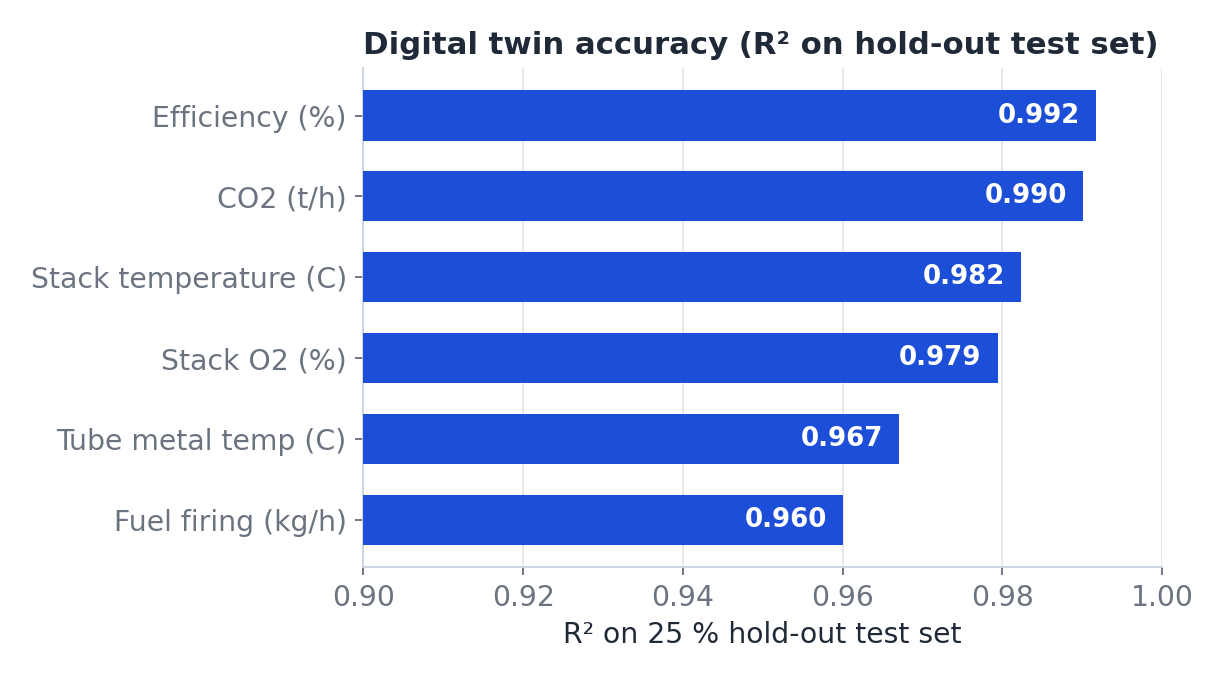
\includegraphics[width=0.82\textwidth]{figures/chart_accuracy.png}
\caption{Twin accuracy per target, all between 0.96 and 0.99, against the
first-principles truth.}
\end{figure}

\begin{figure}[h]
\centering
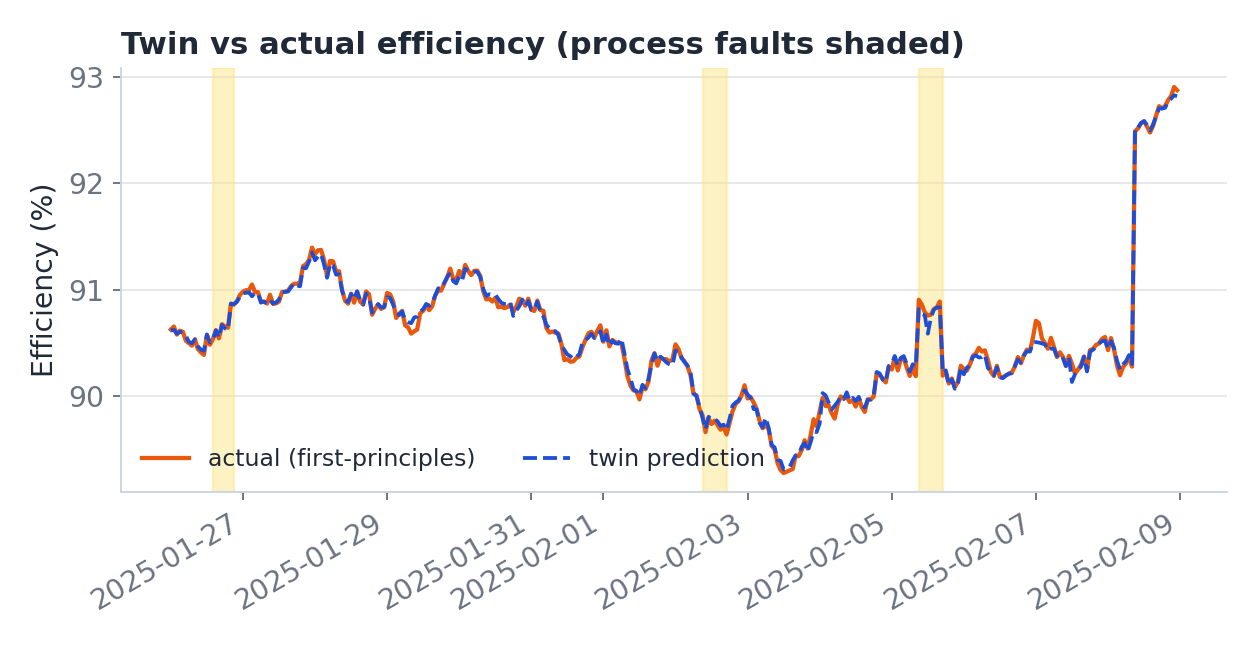
\includegraphics[width=0.92\textwidth]{figures/chart_timeseries.png}
\caption{Predicted efficiency traces the actual efficiency across a fourteen-day
window that includes drift and shaded process faults.}
\end{figure}

%============================ 8. OPTIMIZATION ============================
\section{Operating-point optimization}\label{sec:opt}

The value layer finds the excess-air setpoint that minimises fuel, and therefore
carbon, without crossing the combustion or corrosion limits.

\subsection{Carbon monoxide against excess air}
Below a knee, cutting air lets carbon escape as carbon monoxide. The unburned
fraction is modelled as
\begin{equation}
1-\varepsilon(e) = \min\!\Big(0.03\,\exp\!\big(-(e-0.03)/0.025\big),\ 0.05\Big),
\end{equation}
which gives negligible carbon monoxide above about \SI{12}{\percent} air and a
sharp rise below about \SI{8}{\percent}. This creates a genuine optimum: too much
air wastes heat up the stack, too little makes carbon monoxide.

\subsection{Objective and constraints}
For a fixed duty and fuel, the optimizer sweeps the excess air and selects the
feasible point that minimises the fuel energy $\dot E_f$:
\begin{equation}
\min_{e}\ \dot E_f(e)
\quad\text{s.t.}\quad
CO(e)\le 200\,\si{ppm},\ \
T_s(e)\ge \SI{130}{\celsius},\ \
T_\mathrm{tube}(e)\le \SI{620}{\celsius}.
\end{equation}
The lower stack-temperature bound is the acid dew point, below which the stack
corrodes.

\subsection{Savings and economics}
Comparing the current operation with the optimum gives the savings. With fuel
price $p_f=\SI{6}{USD/GJ}$, carbon price $p_c=\SI{40}{USD/t}$ and $H=8400$
operating hours per year:
\begin{align}
\Delta \dot E_f &= \dot E_f^\mathrm{base}-\dot E_f^\mathrm{opt}, &
\Delta \dot m_{CO_2} &= \dot m_{CO_2}^\mathrm{base}-\dot m_{CO_2}^\mathrm{opt},\\
\text{Fuel value} &= \Delta \dot E_f\, H\, p_f, &
\text{Carbon value} &= \Delta \dot m_{CO_2}\, H\, p_c .
\end{align}

\subsection{Result}
For a representative point currently run at \SI{24}{\percent} excess air, the
optimizer recommends \SI{10}{\percent}, where carbon monoxide just reaches its
limit. Table \ref{tab:opt} summarises the outcome.

\begin{table}[h]
\centering\small
\caption{Optimization result for one heater at the stated prices.}
\label{tab:opt}
\begin{tabular}{@{}lrr@{}}
\toprule
Quantity & Current & Recommended\\
\midrule
Excess air (\si{\percent}) & 24.0 & 10.0\\
Stack oxygen (\si{\percent}) & 4.41 & 2.10\\
Efficiency (\si{\percent}) & 89.40 & 91.89\\
\midrule
\multicolumn{3}{@{}l}{Efficiency gain: \textbf{+2.49 points}}\\
\multicolumn{3}{@{}l}{Fuel saved: \textbf{\SI{2.71}{\percent}} (\SI{5.43}{GJ/h})}\\
\multicolumn{3}{@{}l}{Carbon avoided: \textbf{\SI{2560}{t/yr}}}\\
\multicolumn{3}{@{}l}{Combined value: \textbf{about \SI{376000}{USD} per year, one heater}}\\
\bottomrule
\end{tabular}
\end{table}

\begin{figure}[h]
\centering
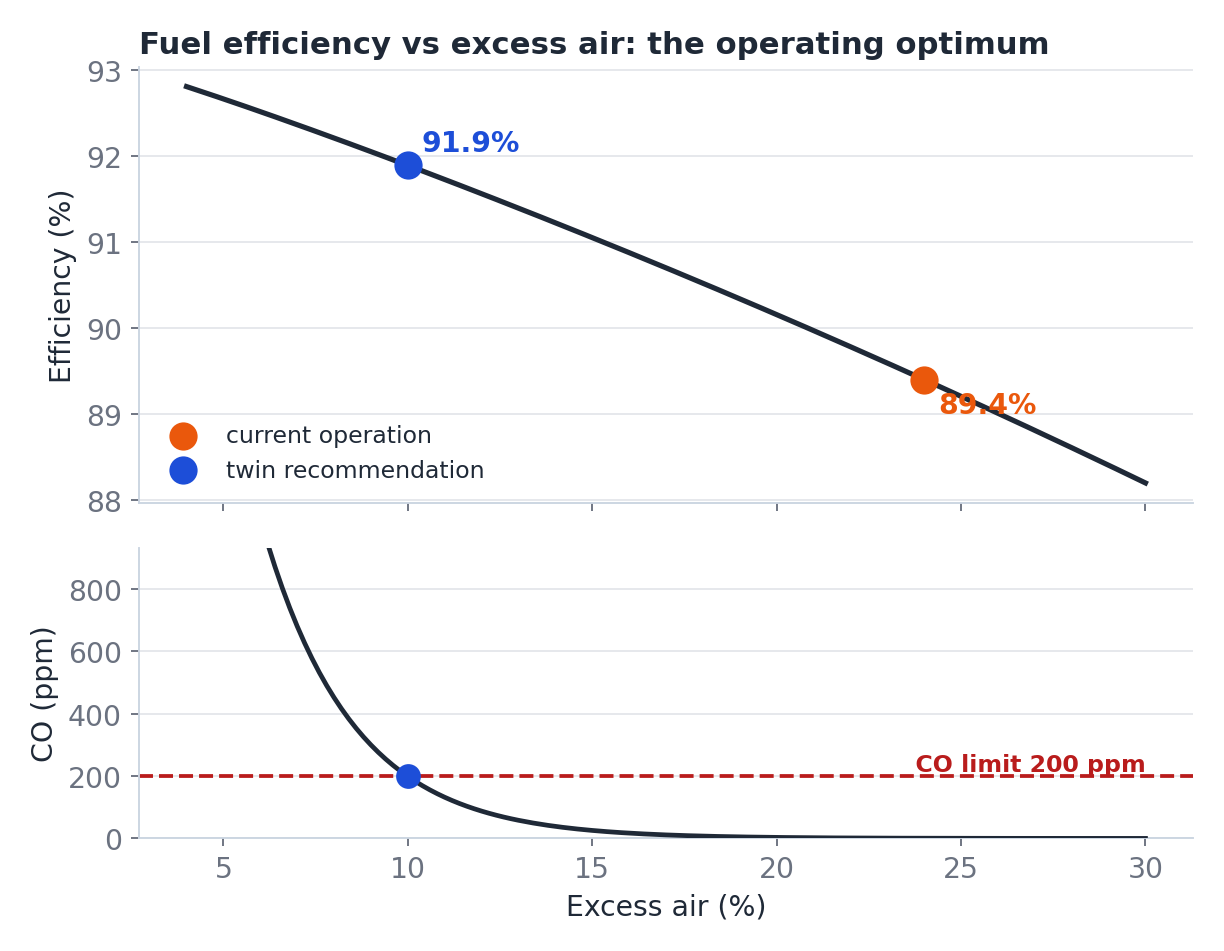
\includegraphics[width=0.86\textwidth]{figures/chart_sweep.png}
\caption{Efficiency against excess air (top) and carbon monoxide against excess
air (bottom). The optimum sits just above the carbon monoxide limit. Orange marks
the current operation, blue the recommendation.}
\end{figure}

%============================ 9. REPRO ============================
\section{Reproducibility}

\subsection{Constants}
\begin{table}[h]
\centering\small
\begin{tabular}{@{}lll@{}}
\toprule
Constant & Symbol & Value\\
\midrule
Process specific heat & $c_{p,p}$ & \SI{2.55}{kJ/(kg.K)}\\
Design stack temperature & $T_s^0$ & \SI{160}{\celsius}\\
Design excess air & $e_0$ & \SI{15}{\percent}\\
Radiant fraction & $f_r$ & 0.70\\
Hot flue specific heat & $c_{p,g}$ & \SI{1.35}{kJ/(kg.K)}\\
Carbon dioxide factor & $F$ & \SI{56.1}{kg/GJ}\\
Refractory loss & & \SI{2}{\percent}\\
Unaccounted loss & & \SI{2.5}{\percent}\\
Fuel price & $p_f$ & \SI{6}{USD/GJ}\\
Carbon price & $p_c$ & \SI{40}{USD/t}\\
Operating hours & $H$ & 8400 per year\\
\bottomrule
\end{tabular}
\end{table}

\subsection{Code map and run order}
\begin{table}[h]
\centering\small
\begin{tabular}{@{}ll@{}}
\toprule
File & Role\\
\midrule
\texttt{fuel\_properties.py} & Sections \ref{sec:fuel}--\ref{sec:comb}: fuel and combustion\\
\texttt{heater\_model.py} & Sections \ref{sec:heater}--\ref{sec:kpi}: energy balance and KPIs\\
\texttt{generate\_dataset.py} & Section \ref{sec:data}: dataset generation\\
\texttt{twin\_pipeline.py} & Section \ref{sec:twin}: clean, label, train, validate\\
\texttt{optimize.py} & Section \ref{sec:opt}: optimizer\\
\texttt{make\_charts.py} & the figures in this report\\
\texttt{dashboard.py} & Streamlit live demo\\
\bottomrule
\end{tabular}
\end{table}

Run order:
\texttt{generate\_dataset.py} $\rightarrow$ \texttt{twin\_pipeline.py} $\rightarrow$
\texttt{optimize.py} $\rightarrow$ \texttt{make\_charts.py} $\rightarrow$
\texttt{streamlit run dashboard.py}.

\section{Assumptions and limitations}

\begin{itemize}[leftmargin=1.4em]
  \item The results come from a first-principles simulation, not a live plant. The
        reported accuracy is the surrogate against the physics model, not against
        field measurements. The next milestone is calibration on a real heater.
  \item The steady-state model resolves one instant at a time and does not capture
        fast transients or detailed burner aerodynamics.
  \item The flame temperature and nitrogen-oxide relations are calibrated
        estimates, adequate for trend and optimization, not for detailed emissions
        design.
  \item The economics use indicative prices. The physical savings, fuel and carbon
        per hour, do not depend on those prices.
\end{itemize}

\end{document}
